\documentclass{report}


\usepackage[table]{xcolor} % Before listings
\usepackage{amsmath} % Better matrix environment
\usepackage{amssymb}
\usepackage[inline]{enumitem} % inline numbering and resume numbering
\usepackage{etoolbox} % If conditions
\usepackage{graphicx}
\usepackage{listings} % for code
\usepackage{nth}
\usepackage{hyperref}
\usepackage{cleveref} % Must be loaded after hyperref
\usepackage{caption}
\usepackage{pgfplotstable}
\pgfplotsset{compat=1.10}
\usepackage{subcaption}
\usepackage{svg}
\usepackage{tikz}
\usepackage{tikz-qtree,tikz-qtree-compat} % Trees
\usepackage{url}
\usepackage{xkeyval}

\pdfoptionpdfminorversion=5

% Squiggly lines
\usetikzlibrary{decorations.pathmorphing}


% Node shapes
\usetikzlibrary{shapes,decorations}

% Coordinate calculation
\usetikzlibrary{calc}

% For charts
\usetikzlibrary{patterns}

\newcommand{\VertexSet}{V}
\newcommand{\CellSet}{C}

\newcommand{\Visited}{V_{visited}}

% Cardinality of
\newcommand{\card}[1]{\left\vert{#1}\right\vert}

% powerset of
\newcommand{\powerset}[1]{\mathcal P \left({#1}\right)}



% Line that can go anywhere, structured region or outside
\tikzset{%
    anywhere/.style={
		decorate,
		decoration={
		    snake,
		    segment length=4,
		    amplitude=.9,post=lineto,
		    post length=2pt
		}
	}
}

% Line that can only go outside the structured region
\tikzset{outside/.style={dotted}}


% Ellipsis
\tikzset{ellipsis/.style={loosely dotted}}



\begin{document}

\chapter{Introduction}
Scientific computing is a large research branch touching on various areas in the scientific community as well as in various industries. An integral part of it is concerned with algorithms and techniques which operate on a mesh representation of a model, typically modelling physical phenomena such as the motion of fluids. SEE
% [Flow simulation and high performance computing, 1996a T. Tezduyar, http://www.tafsm.org/PUB_PRE/jALL/j63-CM96.pdf]
. SEE
% [http://www.sv.vt.edu/classes/MSE2094_NoteBook/97ClassProj/num/widas/history.html]
for a good introduction on finite element analysis.


Various methods of representing meshes exist, including X, Y, and Z
% [http://en.wikipedia.org/wiki/Polygon_mesh#Representations]
. Representations typically rely on encoding some form of explicitly-defined mapping between mesh elements. This can be represented straightforwardly as a flat array, with the array indices representing elements in the source set, and each value being one or more values representing one or more elements in the destination/target set. We focus our attention to the case where the number of target elements mapped to from each source element is constant. Such a map is known as a constant-arity map.

Consider for instance a quadrilateral mesh with two element sets \texttt{C} and \texttt{V}, representing the set of cells and vertices, respectively.
We can define a dat of coordinates, which associates the set each vertex $v \in V$ with a coordinate pair $(x_v, y_v)$, representing its position in 2D space.

We can then define an adjacency map (of constant arity 4) from cells to vertices:

\texttt{$C \rightarrow Node^4$}

Now consider an operation over this mesh, which performs a computation for each cell $c \in C$ as a function of its adjacent nodes ${n | n \in Map[c]}$, for instance computing the area of the cell. In particular consider the chain of memory access indirections and the resulting memory access patterns:

%
%             |   |             |   |
%             |   |  /----n3--->|   | -> (x_1, y_1)
%             |   | /           |   |
% cell_id ->  |   |/------n1--->|   | -> (x_4, y_4)
%             |   |\            |   |
%             |   | \-----n4--->|   | -> (x_5, y_5)
%             |   |  \          |   |
%             |   |   \---n2--->|   | -> (x_12, y_12)
%             |   |             |   |
%             |   |             |   |
%             |   |             |   |
%           cell2nodes         node2coordinate

Notice that proximate (or indded adjacent) nodes in the mesh need not exhibit a uniform memory access pattern. This is detrimental to performance for various reasons.
1. They do not exhibit spatial locality, a property which most modern CPU caches bank on to attain higher performance in IO bound applications, which may manifest through decisions regarding cache replacement strategies or data pre-fetching.
2. Looking up addresses, as opposed to computing them directly, will typically prohibit or limit the scope of compiler-performed optimizations, not least vectorizations.

Numerous strategies have been devoted to deal with this problem, notably applying a space filling curve to obtain a more favourable numbering, with closer elements tending to have closer numberings. While the space filling curve most certainly improves cache locality, it does not make use more obvious structure that may exist. A mesh that is irregular and unstructured on the whole may contain subregions of high regularity and uniform structure, whose regularity/uniformity may be locally exploitable in a more direct manner, for potentially higher gain!


We present Crystal mesh, a group of algorithms for \emph{extracting} regions of regularity in a mesh, reorganizing the mesh to \emph{expose} said structure in order to enable efficient \emph{exploitation}.
In particular, we present and evaluate an implementation for extracting and exposing structure in quadrilateral meshes on various examples, and evaluate a 33\% performance improvement achieved by exploiting the structure on the airfoil computation.


\chapter{Background}
\section{The mathematical mesh model}

Meshes often model physical objects and phenomena. This is typically achieved through the discretization of a continuous model, such as the surface or volume of an object, in order to approximate its physical properties to a desired degree of precision.
\par

The mesh model consists of a hierarchy of elements, which may include a subset the following:
\begin{itemize}
\item Polyhedra such as cubes or tetrahedrons
\item Polygons \emph{(also referred to as cells or faces)} such as triangles and quadrilaterals
\item Edges
\item Vertices \emph{(also referred to as nodes)}
\end{itemize}

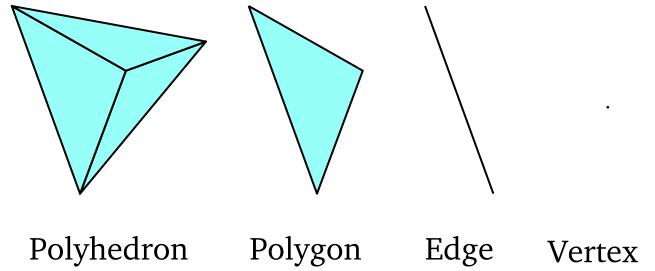
\includegraphics[scale=0.5]{images/background/mesh-elements.pdf}

Each element in the above hierarchy is built-up from those below it. Thus, a polyhedron is assimilated by a set of polygons, a polygon is composed by a set of edges, and an edge joins two vertices.


\subsection{Geometry vs topology}
There is a key distinction to make between the geometric and topological properties of a mesh.

Since meshes model a physical reality, the elements of a mesh may be spatially embedded: vertices are associated with points in space, and edges are formed as segments joining their two vertices. This affects \emph{geometric} properties of the mesh, such as its surface area or volume.

On the other hand, the hierarchy of elements described above induces a mesh topology. This describes the connectedness of the mesh, that is to say how elements relate to one another. For instance, we may describe two vertices sharing an edge as \emph{adjacent}, or two cells being \emph{incident} on an edge.
\par
In this work we concern ourselves solely with the topological structure of meshes, treating its geometry as arbitrary data that is associated with its respective elements (the position of a vertex for instance). Figure~\ref{fig:same-topology} illustrates the difference between the two concepts.

\begin{figure}
    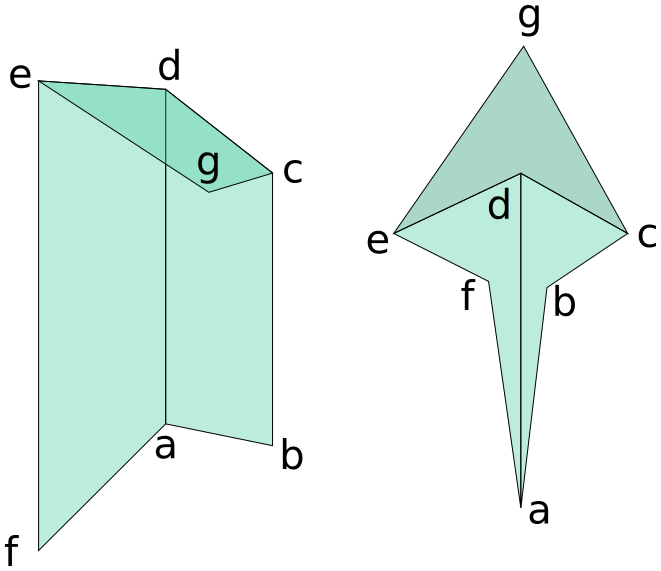
\includegraphics[scale=0.5]{images/background/same-topology.pdf}
    \caption{Despite having completely different geometric shapes and properties, the two meshes are topologically equivalent. The labels indicate corresponding vertices.}
    \label{fig:same-topology}
\end{figure}




\subsection{Manifold meshes}
A mesh is a manifold if the following properties hold:
\begin{enumerate}
\item All edges are adjacent to either one or two faces.

\item All faces meeting at a given vertex must form either an open or a closed fan around that vertex (Figure~\ref{fig:open-closed-fans}).
\end{enumerate}

% Open and closed fans
\begin{figure}
    \sidebyside
        {\includegraphics[scale=0.2]{images/background/closed-fan.pdf}
        \caption{A closed fan}}
        {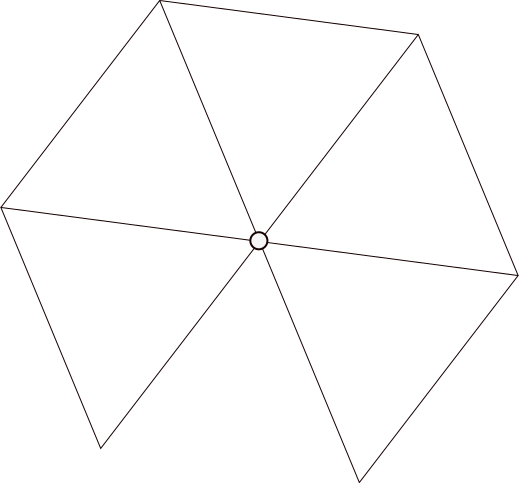
\includegraphics[scale=0.2]{images/background/open-fan.pdf}
        \caption{An open fan}}
    \caption{}
    \label{fig:open-closed-fans}
\end{figure}

Figure~\ref{fig:non-manifolds} demonstrates examples of non-manifold meshes.

% Non-manifolds
\begin{figure}
    \sidebysidefour
    {\includegraphics[scale=0.2]{images/background/bad-fan.pdf}
        \caption{Faces incident on a vertex which do not form a continuous fan}}
    {\includegraphics[scale=0.2]{images/background/bad-fan2.pdf}
        \caption{An extra face that breaks off from the otherwise closed fan}}
    {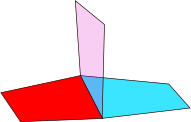
\includegraphics[scale=0.8]{images/background/bad-multi-edge.pdf}
        \caption{More than two faces incident on a single edge}}
    {\includegraphics[scale=0.8]{images/background/bad-no-edge.pdf}
        \caption{An edge with no incident faces}}

    \caption{Examples of non-manifold meshes.}
    \label{fig:non-manifolds}
\end{figure}

In this work we consider manifold meshes exclusively, and future mentions of `mesh' shall implicitly refer to manifold meshes.




\section{The mesh data structure}

We describe how a mesh model is manifest at the data structure level. There are three general component types can be identified:
\begin{itemize}
\item Entity sets
\item Associative data
\item Relations between two entity sets
\end{itemize}

In the following sections, the examples shall refer to the mesh depicted in figure~\ref{fig:example-mesh}.

\begin{figure}
    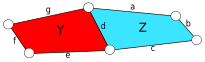
\includegraphics[scale=2]{images/background/mesh-data-structure.pdf}
    \caption{Example mesh with labelled elements.}
    \label{fig:example-mesh}
\end{figure}


\subsection{Entity sets}
Each set represents a certain type of entity in the mesh, such as vertices or cells. Each element in a set is associated with a unique identifier. Integers are a common choice as an identifier for a couple of reasons:
\begin{itemize}
\item They need not be enumerated explicitly. All we need is the set cardinality and a starting index.
\item They are convenient for direct-indexed array accesses, as well as for more general indexing methods.
\end{itemize}

See figure~\ref{fig:entity-sets} for examples.

\begin{figure}
    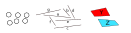
\includegraphics[scale=4]{images/background/entity-sets.pdf}
    \caption{The entity sets of the mesh in figure~\ref{fig:example-mesh}. These are (from left to right) the vertices, edges, and cells.}
    \label{fig:entity-sets}
\end{figure}


\subsection{Associative data}
Arbitrary data which is associated with elements of a particular entity set. For instance, spatial coordinates associated with each vertex. A typical representation is a flat array indexed by element identifier.
This is the data over which we perform our computations and ultimately care about. Everything else is incidental.

See figure~\ref{fig:associative-data} for an example.

\begin{figure}
    
\includegraphics[scale=4]{images/background/associative-data.pdf}
    \caption{Coordinate data associated with the vertices of the mesh in figure~\ref{fig:example-mesh}.}
    \label{fig:associative-data}
\end{figure}


\subsection{Relation maps between two entity sets}
Entity sets may have relations defined between them, a mapping from an element in a source set to one or more corresponding elements in the destination set. For instance, we may have an adjacency relation from the vertex set to itself, or an inclusion relation from the cell set to the vertex set.
In a general unstructured mesh these relations must be explicitly stored, typically as an array indexed by the source element's identifier.

See figure~\ref{fig:relation} for an example.

\begin{figure}
    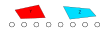
\includegraphics[scale=4]{images/background/relation.pdf}
    \caption{Inclusion relation from cells to vertices, as depicted in the mesh of figure~\ref{fig:example-mesh}.}
    \label{fig:relation}
\end{figure}




\section{The mesh core-computation contract}
Given a mesh model and its underlying representation, computation logic provided by an external user is to be executed. We refer to this as the \emph{core-computation}; this is to disambiguate it from other incidental processing, such as structure detection.
Our contract to the user is described in what follows.

\subsection{Given: entity set}
We are given an entity set over which to operate, for example the set of edges or the set of cells. The core-computation consists of executing a computation for each element of this set. This is analogous to the \emph{map} phase of the MapReduce programming model\footnote{REFERENCE}, though we restrict our usage of the term \emph{map} to refer to relation maps.

\subsection{Given: relation-map tree}
We are given a tree structure defining which relation maps to use and how to access them. This is best explained through an example, illustrated in figure~\ref{fig:relation-tree}.


\begin{figure}
    %% Key icon
    \newcommand{\keyicon}{
\includegraphics[width=6pt]{images/background/key.pdf}}

    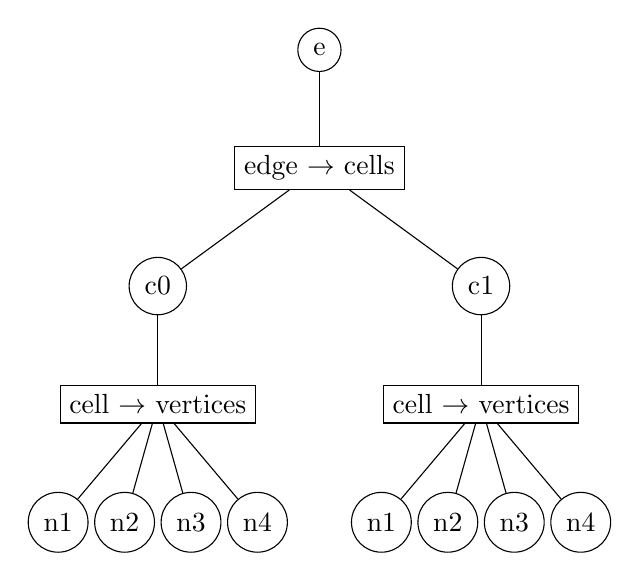
\begin{tikzpicture}[every tree node/.style={draw,circle},
        level distance=1.5cm,
        edge from parent path={(\tikzparentnode) -- (\tikzchildnode)}]

    \tikzset{level 2/.style={sibling distance=0.8cm}}

    \Tree
    [.{e}
        \edge node[auto=right] {\keyicon};
        [.\node[rectangle] {edge $\rightarrow$ cells};
            [.{c0}
                \edge node[auto=right] {\keyicon};
                [.\node[rectangle] {cell $\rightarrow$ vertices};
                    [.n1 ]
                    [.n2 ]
                    [.n3 ]
                    [.n4 ]
                ]
            ]
            [.{c1}
                \edge node[auto=right] {\keyicon};
                [.\node[rectangle] {cell $\rightarrow$ vertices};
                    [.n1 ]
                    [.n2 ]
                    [.n3 ]
                    [.n4 ]
                ]
            ]
        ]
    ]
    \end{tikzpicture}
    \caption{EXPLANATION}
    \label{fig:relation-tree}
\end{figure}





% \item The entity set over which to operate.
% \item Any relation maps to follow, and the variables by which they are indexed. Indexing variables may include the current iteration element, as well as the targets got by following another map.
% In general this may involve complex chains of maps, though only up to to two levels of indirection are used in practice.
% \item A kernel function which is to be applied to each element in the given entity set.
% \end{itemize}

A \emph{kernel function} specifying the computation logic is given. This kernel function is associated with a particular entity set.

The execution contract

When performing some computation over a mesh, the data access pattern followed is typically as follows:
\begin{enumerate}
\item Iterate over the elements of an entity set, in no particular order.
\item For each element iterated over, gather any handles to associated elements (the indices of adjacent elements, say). This may involve handles obtained through a chain of set relationship maps.
\item Access the associative data using the gathered handles.
\end{enumerate}


 The computation is often specified as a \emph{kernel function} operating a particular entity set



\chapter{Related works}
% \section{Structure is beneficial}



% - How do quad meshes with subregions of structure come about
% - Are they seen often


\section{Structure detection and extraction}


% Fast Neighborhood Search on Polygonal Meshes
% http://www.inf.ethz.ch/personal/dpanozzo/papers/EGIT11-RocDeGPanPup.pdf
% Dude et al tackle the specific problem of neighborhood search by defining a spatial index, a hierarchy of clusters of vertices. Their method yields an approximation, ours is exact, with the mesh model left completely unaltered. However, we can learn a few things.

% The problem of indirections and its derivatives (non-contiguous memory access and its impact on cache hierarchy) is cited/highlighted as a key motivation in basing their mesh data structure on a geometric model, i.e. the spatial index. We undertake the opposite approach, viewing geometric data as mere associative data attached to a topological mesh model.

Adapting the mesh model to use a structured representation for the benefit of the relevant application domain is (not new) / (fairly prevalent).
Rocca et al.~\cite{rocca2011fast} address the particular problem of neighbourhood search: finding the set of vertices within a certain distance from a given vertex. They define a spatial index, a hierarchy of vertex clusters, that yields good approximations to neighbourhood search queries.

The problem of memory access indirections, associated with representing the mesh topology, is cited as a key motivation for basing their mesh data structure (the aforementioned spatial index) on a geometric model which does not require storing topological information. This is in sharp contrast to our approach of transforming the mesh topology representation, and treating the mesh geometry as arbitrary associative data.



% Motorcycle Graphs: Canonical Quad Mesh Partitioning
% http://www.ics.uci.edu/~goodrich/pubs/geomproc.pdf
% Whilst the motivations are different (mesh compression AND mesh isomorphism) the approach is similar:
% ``The simplest quadrilateral meshes are structured meshes, in which connections between quadrilaterals form a regular grid, but in complicated domains it may be necessary to use semi-regular meshes in which this structure is interrupted by a small number of extraordinary vertices that do not have degree four. We study how to partition a semi-regular mesh into a small number of structured submeshes.''


% ``To ensure that isomorphisms will always be found when they exist, our partition must be canonical: the same mesh must always generate the same partition. The partitioning algorithm we describe has this property.''
% We do not care about this property per se. There may be multiple optimal solutions for structure detection, for example.


% ``Additionally, these techniques may apply to areas beyond graphics such as scientific computation. Code for the finite element method can be greatly streamlined when applied to structured quadrilateral meshes. By partitioning unstructured meshes into structured submeshes, it should be possible to achieve similar speedups for semi-regular meshes.''

Eppstein et al.~\cite{eppstein2008motorcycle} describe a method for partitioning quadrilateral meshes into structured regions using the \emph{motorcycle graph} construction, whose inspiration came from the 1982 movie Tron. The algorithm works by placing particles on each \emph{extraordinary} vertex\footnote{\label{footnote:extraordinary-vertices} This is in contrast to an \emph{ordinary} vertex, which the authors define as ``a non-boundary vertex incident with four edges or a boundary vertex incident with at most three edges.''} in the mesh, and advancing them along edges until they collide. The enclosed regions formed by the paths represent structured regions.

Whilst the motivations are different, with the emphasis on applications in mesh compression and detecting mesh isomorphisms, the approach may be applicable to the scientific computation domain. Indeed, the authors state this explicitly:
\begin{quote}
These techniques may apply to areas beyond graphics such as scientific computation. Code for the finite element method can be greatly streamlined when applied to structured quadrilateral meshes. By partitioning unstructured meshes into structured submeshes, it should be possible to achieve similar speedups for semi-regular meshes.
\end{quote}

We note, however, that the method makes a stronger assumption about the mesh, in that its ``structure is interrupted by a \emph{small number} of extraordinary vertices that do not have degree four [emphasis added]''.


% There exist processes which explicitly attempt to produce semi-structured meshes, for example *BELOW* which uses domain specific knowledge about the source object to find long strips which can be made into quads.
% Automatic Decomposition and Efficient Semi-Structured Meshing of Complex Solids
% http://www.imr.sandia.gov/papers/imr20/Makem.pdf

Makem et al.~\cite{makem2012automatic} utilise properties of the modelled object to generate meshes with structured regions inherent. The presented method detects long thin shapes with simply defined geometry, such as length and curvature, and generates an appropriate structured region representing these shapes.



\section{Structure in parallel computation}
There is a plethora of work on mesh partitioning optimised for parallel computation. The techniques presented often frame their objectives around these maxims:
\begin{enumerate}
\item \label{item:maximize-locality} Maximizing intra-partition locality, thereby minimizing cross-partition communication.
\item \label{item:minimize-size} Minimize partition size, subject to it being sufficiently large to counterbalance the communication overheads.
\item \label{item:maximize-number} The partitions should be balanced and plentiful in number, so as to utilise parallelism.
``A parallel computation is often only as efficient as the evenness with which its workload is distributed over the processors in a parallel machine.''
\end{enumerate}

Objective~\ref{item:maximize-locality} is certainly a desirable property for our structured regions, and is in fact precisely what we set forth to perform.
On the other hand, objectives~\ref{item:minimize-size} and \ref{item:maximize-number} are rather misaligned with our needs; indeed, a monolithic structured region spanning the entire mesh would represent the best case for us.

Thus some of the techniques which hold these conflicting\footnote{The objectives are in conflict in our context. These objectives are more suited for their parallel context, naturally} objectives may not be fully compatible, though they undoubtedly offer helpful inspiration.

With that said, extending our techniques towards parallel computation is an obvious future step, and such future works should likely re-evaluate their objectives in lieu of this.



% Guide to Partitioning Unstructured Meshes for Parallel Computing
% http://www.hector.ac.uk/cse/reports/unstructured_partitioning.pdf
% Very briefly describes several tools used for partitioning the mesh

A technical report by Ridley~\cite{ridley2010guide} briefly discusses methods for partitioning a mesh so as to maximize spatial data locality, in other words adjacent elements tend to have memory locations that are close. The partitioning is applied by recursively bisecting the mesh geometrically, such that geometrically close points tend to cluster together. The emphasis of the report is towards improving the performance of parallel computation, but the benefits of partitioning extend to serial processing as well.



% Hierarchical Partitioning Techniques for Structured Adaptive Mesh Refinement Applications
% http://www.s3lab.ece.ufl.edu/publication/jsuper.pdf
% Partitions mesh to exploit parallel computation whilst minimizing communication costs. This is done by \emph{exploiting} the hierarchical structure in a mesh. The approach focuses on partitioning for purposes of parallel computation, which involves a) minimizing communication costs; and b) maximizing locality within partitions. We focus solely on B.
% For **future works**, however, A would come into the picture as well, which would add an interesting dimension to the problem for further exploration.
% ``This scheme uses space filling curves (SFC), which are a class of locality preserving recursive mappings from n-dimensional to 1-dimensional space.''
% ALSO, note that this is *dynamic*. We can do that too in the future? :)

Li et al.~\cite{li2004hierarchical} follow a similar theme of parallel computation, although their methods deal with adaptive mesh refinement, where a mesh is dynamically refined in regions with a high calculation error. The refinement process induces a hierarchical structure, which the presented partitioning algorithms aim to exploit.



% Hierarchical hybrid grids: data structures and core algorithms for multigrid
% http://onlinelibrary.wiley.com/store/10.1002/nla.382/asset/382_ftp.pdf?v=1&t=hw5h84yv&s=bbe650e186f348823036d7426c24bd554ea00c1b

Bergen et al.~\cite{bergen2004hierarchical} employ structure-aware mesh refinement techniques, which construct a hierarchy of structured regions with each iterative refinement to the mesh. It is suggested that different element types, such as edges and faces, refined and stored separately, such that their distinct structuredness can be represented.

Since we use a simple structure representation, we make use of augmented structured regions, with different elements' structured region represented in a hierarchy.



% Stencils and Problem Partitionings: Their Influence on the Performance of Multiple Processor Systems
% http://ieeexplore.ieee.org/ielx5/12/35266/01676980.pdf?tp=&arnumber=1676980&isnumber=35266
% Partitioning a mesh based on its memory-access stencil. Again this is parallel oriented. Could be useful in defining the shape of the map access!

Reed et al.~\cite{reed1987stencils} focus on obtaining partitions best-suited to the \emph{stencil structure} associated with a particular computation, that is its neighbour-access pattern. They derive partition shapes for some common stencil structures, optimised to minimise inter-partition communication costs.

Tang et al.~\cite{tang2011pochoir} present a full-fledged \emph{Pochoir Stencil Compiler}. It specifies a domain-specific language that allows users to write a higher-level specification of a stencil computation embedded in C++ code. The compiler then automatically generates very efficient \emph{cache-oblivious}\footnote{The authors of~\cite{frigo1999cache} define a cache oblivious algorithm as that which ``[does not contain] parameters (set at either compile-time or runtime that can be tuned to optimize the cache complexity for the particular cache size and line length''} parallel loops that execute the stencil computation.

As discussed in subsection~\ref{subsec:given-kernel-function}, this is similar to our approach, where the structured regions are detected on the basis of relation-maps, such as cell-vertex or edge-cell maps.


% \url{https://www.cs.sfu.ca/~bgb2/personal/papers/nand11miccai.pdf}
% Bruv et al describe in [REF] the ``[construction of] curvature based features detectors to detect tube-like and sheet-like structures in DTI [diffusion tensor MRI]''. Differential equation-based methods are applied to characterize the ``'structured-ness'' of various components of the generated image, in terms of feature detection. Our focus is on detecting structuring in a precise manner, rather than a characteristic approach.

% FOR FUTURE WORKS: The differential equation approach may be an interesting tangent for future work, for instance applying it to geometric information to deduce areas of likely structure.


% \url{http://ieeexplore.ieee.org/ielx7/83/6490370/06476010.pdf?tp=&arnumber=6476010&isnumber=6490370}
% Again, approximate/heuristical image-based structure detection. The paper mentions low-level and high-level pattern detection.




% multiblock structured mesh partitioning algorithm
% http://www.geuz.org/pipermail/getdp/2000/000138.html
% Michael sends an email discussing stuff







% Structured Grid Computational Pattern
% (EITHER FROM:
%   Course: CS 4800, Fall 2010, School: Northeastern
%   OR
% Parallel Computing Laboratory - Berkley University)
% http://parlab.eecs.berkeley.edu/wiki/_media/patterns/structuredgrid-2.pdf
% http://view.eecs.berkeley.edu/wiki/Structured_Grids
% Good overview of the benefits of structured regions for computation.



\section{Exploiting structure}

% Approximate Topological Matching of Quadrilateral Meshes
% http://www.ics.uci.edu/~goodrich/pubs/approx-match.pdf
% Find matching subgraphs of two meshes, that is having the same topology.

% ``Our reason for using mesh compression instead is based on the desire to speed up the computation time in an algorithm that operates on quad meshes. Thus, our approach actually fits the spirit of other algorithms (e.g., see (33; 15; 14; 38)) that perform data compression so as to improve algorithmic performance.''
% Mentions reducing mesh representation for the purpose of improving computation time.


Eppstein et al.~\cite{eppstein2008approximate} explore the problem of approximate topological matching between given quadrilateral meshes, that is detecting isomorphisms between their submeshes. To this end they discuss various techniques based on \emph{particle shooting}\footnote{The motorcycle graph construction discussed in the paper by the same authors~\cite{eppstein2008motorcycle} is based on particle shooting.}: ``particles'' are placed on certain vertices (for example, extraordinary vertices\footref{footnote:extraordinary-vertices}) and are then ``'fired'' along the mesh using certain rules.

One such algorithm, termed ``The Greedy Algorithm'' by the authors, is shown to suffer from a problem when particles advancing along the same front can get out of sync. The problem is remarkably similar to our discussion about contiguous detection in subsection~\ref{subsec:contiguous-detection}.


% Opportunistic Data Structures with Applications
% http://people.unipmn.it/manzini/papers/focs00draft.pdf
% Discusses implicit data structures which minimize storage overheads due to auxiliary information


% \section{}


% Predictable memory access patterns versus *known* memory access pattern.



**** POINT OF MENTION:
Applying our structure detection algorithm to meshes with intentional structure is still useful, as it provides an efficient, automatic method of generating a mesh and the associated code to run exploiting that structure.


\chapter{Diving into the problem}

\section{A basic definition of structure}
What we would like is a form of structure which is
\begin{enumerate*}[label=\alph*)]
\item representable as a data structure, and \item efficient in terms of performance.
\end{enumerate*}

Given our semantic knowledge about the mesh model we can ascertain some facts about relationship maps:
\begin{itemize}
\item They are sparse: element arity is very small compared to the number of elements, and is in fact unrelated to it.
\item They have a high clustering coefficient: Relationships tend to be localized, forming tightly connected clusters.
% TODO REFERENCE TO CLUSTERING COEFFICIENTS
\end{itemize}

These properties arise as a consequence of meshes modelling real-world phenomena that exist in a Cartesian space.
On this basis, we consider a spatial embodiment of element relationships, organising the elements in a discrete space such that the uniform relationship is apparent.

Bear in mind that this approach carries no relation to any geometric data associated with elements, such as the coordinates of vertices. To make this distinction clear, as well as to emphasize its discrete nature, we address this Cartesian-like space by rows and columns rather than x and y coordinates.

\subsection{Example: Naca0012 mesh}
Below is a small extract from the NACA0012 mesh\footnote{Thanks to Dr. Peter Vincent, George Ntemos and Harry Davis}, showing the cross section of an aerofoil mesh and its interaction with surrounding fluid. The mesh is divided into cells which represent the ...

\newcommand{\drawnaca}[2]{
	% trim left bottom right top
	\includesvg[svgpath=#1]{#2}
}
\drawnaca{images/defining-structure/}{naca0012-plain}

The vertices in the highlighted region seem like good candidates for a ``structured region'', forming a two-dimensional lattice in a discrete Cartesian space. This ``structured region'' has the properties outlined below.

\subsection{Properties of a structured region}
\label{sec:structured-region-properties}
\begin{enumerate}
\item All vertices have a uniform arity of four.
\item Every vertex has a consistent discrete direction (for example the cardinal directions: north east, south, west) with respect to the other vertices. In other words, the direction is transitive: if vertex $a$ is above vertex $b$, and vertex $b$ is above vertex $c$, then vertex $a$ is above vertex $c$. As a non-example, consider this case:
** INSERT IMAGE AND EXPLANATION **
\end{enumerate}


\drawnaca{images/defining-structure/}{naca0012-node-structure}

%% TODO Maybe not introduce data structure yet????
We can propagate this inherent structure from the mesh model to the underlying data structure, representing this two-dimensional lattice using a two-dimensional array. Vertices may be assigned Cartesian coordinates, but in spirit of the space's discreteness we shall use rows and columns instead.

\drawnaca{images/defining-structure/}{naca0012-node-grid}


\newcommand{\strV}{V_{str}}
\newcommand{\adjstrV}{V_{adjstr}}
\newcommand{\AdjVVstr}{Adj_{\adjstrV\strV}}

Let us call $\VertexSet$ the set of all vertices, and $\strV \subseteq \VertexSet$ the set of vertices in the ``structured region''.

\subsection{Representing the vertex-vertex adjacency}

Now consider the vertex-vertex adjacency relation $\AdjVV: \VertexSet \mapsto \VertexSet$ in context of the ``structured region'' $\strV$. We can directly locate a particular neighbour of any vertex, for example its north neighbour, so long as that neighbour is also within the structured region. This restricts the set of vertices with fully-accessible neighbours to those which are not on the borders of the ``structured region''. This is the subset of vertices $\adjstrV \subseteq \strV$ which are structured \emph{with respect to} $\AdjVV$. This induces a new relation which operates purely within the structured region:
$$\AdjVVstr: \adjstrV \mapsto \strV$$

\drawnaca{images/defining-structure/}{naca0012-node-neighbours}


\definecolor{neighbourstructurecolor}{RGB}{174,190,226}

% Draw structured node region
\begin{tikzpicture}[scale=0.7]
	\newcommand{\stylewithfill}[1]{\tikzstyle{every node}=[draw, shape=circle, minimum size=0.8cm, fill=#1];}
	\stylewithfill{none}

	% ROW 0
	\drawgrid{rows=1, cols=3, rowoffset=0, coloffset=4, labeler=\plainlabelnode, labelerA=0, labelerB=2,
		southborder=structured}

	% ROW 1
	\drawgrid{rows=1, cols=2, rowoffset=-2, coloffset=0, labeler=\plainlabelnode, labelerA=1, labelerB=0,
		eastborder=structured}

	{
	\stylewithfill{neighbourstructurecolor}
	\drawgrid{rows=1, cols=2, rowoffset=-2, coloffset=4, labeler=\plainlabelnode, labelerA=1, labelerB=2,
		northborder=structured, southborder=structured, westborder=structured, eastborder=structured}
	}

	\drawgrid{rows=1, cols=1, rowoffset=-2, coloffset=8, labeler=\plainlabelnode, labelerA=1, labelerB=4,
		northborder=structured, southborder=structured, westborder=structured}


	\drawgrid{rows=1, cols=1, rowoffset=-2, coloffset=12, labeler=\plainlabelnode, labelerA=1, labelerB=6,
		southborder=structured, eastborder=structured}

	\drawgrid{rows=1, cols=1, rowoffset=-2, coloffset=14, labeler=\plainlabelnode, labelerA=1, labelerB=7,
		westborder=structured}

	% ROW 2
	\drawgrid{rows=1, cols=1, rowoffset=-4, coloffset=4, labeler=\plainlabelnode, labelerA=2, labelerB=2,
		northborder=structured, southborder=structured, eastborder=structured}

	{
	\stylewithfill{neighbourstructurecolor}
	\drawgrid{rows=1, cols=2, rowoffset=-4, coloffset=6, labeler=\plainlabelnode, labelerA=2, labelerB=3,
		northborder=structured, southborder=structured, eastborder=structured, westborder=structured}
	}

	\drawgrid{rows=1, cols=1, rowoffset=-4, coloffset=10, labeler=\plainlabelnode, labelerA=2, labelerB=5,
		southborder=structured, westborder=structured, eastborder=structured}

	\drawgrid{rows=1, cols=1, rowoffset=-4, coloffset=12, labeler=\plainlabelnode, labelerA=2, labelerB=6,
		northborder=structured, westborder=structured}

	% ROW 3
	\drawgrid{rows=1, cols=1, rowoffset=-6, coloffset=4, labeler=\plainlabelnode, labelerA=3, labelerB=2,
		northborder=structured, southborder=structured, eastborder=structured}

	{
	\stylewithfill{neighbourstructurecolor}
	\drawgrid{rows=1, cols=2, rowoffset=-6, coloffset=6, labeler=\plainlabelnode, labelerA=3, labelerB=3,
		northborder=structured, southborder=structured, eastborder=structured, westborder=structured}
	}

	\drawgrid{rows=1, cols=1, rowoffset=-6, coloffset=10, labeler=\plainlabelnode, labelerA=3, labelerB=5,
		northborder=structured, westborder=structured}

	% ROW 4
	\drawgrid{rows=1, cols=1, rowoffset=-8, coloffset=2, labeler=\plainlabelnode, labelerA=4, labelerB=1, eastborder=structured}

	{
	\stylewithfill{neighbourstructurecolor}
	\drawgrid{rows=1, cols=2, rowoffset=-8, coloffset=4, labeler=\plainlabelnode, labelerA=4, labelerB=2,
		northborder=structured, southborder=structured, eastborder=structured, westborder=structured}
	}

	\drawgrid{rows=1, cols=1, rowoffset=-8, coloffset=8, labeler=\plainlabelnode, labelerA=4, labelerB=4,
		northborder=structured, westborder=structured}

	% ROW 5
	\drawgrid{rows=1, cols=2, rowoffset=-10, coloffset=4, labeler=\plainlabelnode, labelerA=5, labelerB=2,
		northborder=structured}
\end{tikzpicture}

The key insight we make is that for structured regions in a mesh we need not represent set relationship maps explicitly; the uniformity of set relations allows us to deduce the relationships. We can encode the relation $\AdjVVstr$ very simply. Given a vertex $n_{r,c} \in \adjstrV$, located at row $r$ and column $c$, its four vertex neighbours are $n_{r,c-1}$, $n_{r,c+1}$, $n_{r-1,c}$, and $n_{r+1,c}$.



% Draw structured node region
\begin{tikzpicture}[scale=1]
	\newcommand{\stylewithfill}[1]{\tikzstyle{every node}=[draw, shape=circle, minimum size=1.3cm, fill=#1];}
	\stylewithfill{none}

	% ROW 0
	\drawgrid{rows=1, cols=1, rowoffset=0, coloffset=2,
		labeler=\varlabelnode, labelerA=-1, labelerB=0, labelerC=r, labelerD=c,
		southborder=structured}

	% ROW 1
	\drawgrid{rows=1, cols=1, rowoffset=-2, coloffset=0,
		labeler=\varlabelnode, labelerA=0, labelerB=-1, labelerC=r, labelerD=c,
		eastborder=structured}

	{
		\stylewithfill{neighbourstructurecolor}
		\drawgrid{rows=1, cols=1, rowoffset=-2, coloffset=2,
			labeler=\varlabelnode, labelerA=0, labelerB=0, labelerC=r, labelerD=c,
			eastborder=structured, westborder=structured, northborder=structured, southborder=structured}
	}

	\drawgrid{rows=1, cols=1, rowoffset=-2, coloffset=4,
		labeler=\varlabelnode, labelerA=0, labelerB=1, labelerC=r, labelerD=c,
		westborder=structured}

	% ROW 2
	\drawgrid{rows=1, cols=1, rowoffset=-4, coloffset=2,
		labeler=\varlabelnode, labelerA=1, labelerB=0, labelerC=r, labelerD=c,
		northborder=structured}

\end{tikzpicture}


\section{Mesh structure as a data structure}
The choice of data structure to represent the structured region is a key one, touching on various aspects:
\begin{itemize}
\item Scope of structure representation: what level of structure can be represented.
\item Implementation complexity of structure detection: how complex a detection algorithm is required.
\item Runtime performance of structure detection: the time and space complexity of the detection algorithm.
\item Storage requirements for detected structure: the storage requirements for the detected structure.
\item Runtime performance of computation over the structured region.
\end{itemize}

We analyse several possible data structure representations.

\subsection{Structure bit map}

\newcommand{\drawbitmap}[2]{
	% trim left bottom right top
	\includesvg[svgpath=#1]{#2}
}

Represent the bounding box around the structured region as a two-dimensional bit map, with each bit representing a vertex position in the superimposed grid. An \emph{on} bit indicates that the corresponding vertex is part of the structured region, an \emph{off} bit otherwise.

\drawbitmap{images/bitmap-representation/}{plain-bitmap}

A bit map can represent \emph{any} structured region which adheres to the properties listed in section~\ref{sec:structured-region-properties}. They are very flexible, capable of representing complex formations as well as handling small anomalies in structure.

Let us define the \emph{efficiency} $\epsilon$ of a bit map as the percentage of its bits which are \emph{on}, as the \emph{off} bits represent wasted vertices. Bit maps with high $\epsilon$ are favourable for several reasons:
\begin{itemize}
\item \emph{Off} bits increase the storage space of the structured region, up to $O(\card{\VertexSet})$ in the worst case, as opposed to $O(\card{STRUCTURED VERTICES})$.
\item \emph{Off} bits similarly worsen the runtime performance, again up to $O(\card{\VertexSet})$ due to wasted execution.
\end{itemize}

A detection algorithm would likely be implemented using a variant of a general graph search algorithm such as breadth-first search or depth-first search. Further consolidation work may be needed to compact disconnected structured components in order to maximize $\epsilon$.
\drawbitmap{images/bitmap-representation/}{disjoint-bitmap}
\drawbitmap{images/bitmap-representation/}{disjoint2-bitmap}



\subsection{Row-specific boundaries}

Represent the structured region as a sequence of consecutive fixed-length rows, permitting vertices outside the structured region to cluster at the beginning and ends of each row. A structured region is then represented by the row-length, as well as individual begin and end offsets for each row.

\drawbitmap{images/per-row-representation/}{plain-per-row}

Storing row-specific boundaries reduces the storage requirement by the order of row-length times.
No executions are wasted as the loop iterations are constrained to vertices in the structured region.
A detection algorithm can be implemented as a simple row-by-row traversal in linear time and space.


On the downside, this scheme trades some of the flexibility offered by the bit map representation, in particularly anomalies in structure which do not occur at the boundaries.


\subsection{Full rectangle}

Represent the structured region as a rectangle of given length and width, with all elements corresponding strictly to vertices within the structured region. The structured region is thus simply represented by the length and the width: the number of rows and the number of columns.

The storage requirement is now constant with respect to the size of the structured region.
Loop iterations are fixed for each region, enabling further optimisation opportunities.
A detection algorithm, as above, can be implemented as a simple row-by-row traversal.

On the downside, the scope of structure representable is limited, being only capable of representing rectangles proper.


\chapter{Rectangle growth strategy}
This chapter covers the detection of rectangular structured regions.

An abstract discussion of various properties of algorithms is presented, and the desirable traits brought forth by each.
Then, a selection of concrete algorithms are described, and their merits and weaknesses examined.


\section{Key concepts}
An \emph{absolute structured position} refers to the position of a structured element with respect to the boundaries of its structured region.
A \emph{relative structured position} refers to the position of a structured element with respect to other structured elements within its structured region. Figure~\ref{fig:structured-position} shows this through an example.


%% Relative vs absolute
\begin{figure}
\newcommand{\nodesize}{1.2}
\newcommand{\rows}{4}
\newcommand{\cols}{4}
\newcommand{\rowsize}{\rows*\nodesize}
\newcommand{\colsize}{\cols*\nodesize+2*0.1}

% Node at position r, c, label
\newcommand{\nodeat}[3]{
	\pgfmathsetmacro{\lerow}{ (\rows - #1) * \nodesize - (\nodesize / 2) - 0.1}
	\pgfmathsetmacro{\lecol}{ (#2 * \nodesize) + (\nodesize / 2) + 0.1}
	\node at (\lecol, \lerow) {#3}
}

\sidebyside
{
	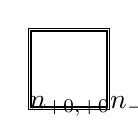
\begin{tikzpicture}
		\tikzstyle{every node}=[draw, shape=rectangle, minimum size=\nodesize cm, font=\small];
		\draw[double] (0,0) rectangle (\colsize,\rowsize);
		\nodeat{2}{1} {$n_{+0,+0}$};
		\nodeat{1}{1} {$n_{-1,+0}$};
		\nodeat{2}{2} {$n_{+0,+1}$};
	\end{tikzpicture}
	\caption{Relative structured position\label{fig:relative-structured-position}}
}
{
	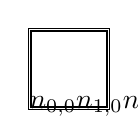
\begin{tikzpicture}
		\tikzstyle{every node}=[draw, shape=rectangle, minimum size=\nodesize cm, font=\small];
		\draw[double] (0,0) rectangle (\colsize,\rowsize);
		\nodeat{0}{0} {$n_{0,0}$};
		\nodeat{1}{0} {$n_{1,0}$};
		\nodeat{0}{1} {$n_{0,1}$};
	\end{tikzpicture}
	\caption{Absolute structured position\label{fig:absolute-structured-position}}
}
\caption{Depiction of \emph{relative} structured position versus \emph{absolute} structured position. The row and column counts are increasing down and to the right, respectively. The borders indicate structured regions, whose origin resides in the top-left corner.\label{fig:structured-position}}
\end{figure}



\section{Properties of detection algorithm}

\subsection{Eager detection}
An eager (or greedy) detection algorithm will include every structured element if finds immediately, regardless of the long term consequences. While this strategy may lead to suboptimal results, it avoids backtracking the structure detection which may be prohibitively costly.


\begin{figure}
\pgfplotstableread{
	2 2 2 2 2 2 0
	2 2 1 2 2 0 0
	0 0 1 0 0 0 0
	0 0 1 0 0 0 0
}{\eagermatrix}
\pgfplotstableread{
	2 2 2 2 2 2 0
	2 2 0 2 2 0 0
	1 1 1 1 1 1 1
	1 1 1 1 1 1 1
}{\noneagermatrix}

\sidebyside
{
	\drawmatrix[cell wd=0.6, cell ht=0.6]{\eagermatrix}
	\caption{Eager detection may greedily add the northern cell, yielding a suboptimal structured region.}
}
{
	\drawmatrix[cell wd=0.6, cell ht=0.6]{\noneagermatrix}
	\caption{A non-eager algorithm could instead decide to ignore the northern cell, yielding a larger structured region.}
}
\caption{Eager versus non-eager detection. Black cells and white cells denote unstructured and structured elements, respectively. Red cells denote structured elements detected as forming a rectangular structured region.}
\end{figure}



\subsection{Contiguous detection}
An algorithm which exhibits continuous detection always adds a structured element which is contiguous to the structured region thus far. The implication is that the relative structured position is always known. This greatly simplifies detection, as all adjacent structured elements are known at any point in time, and structured elements need not be repositioned in the structured region.

In the case of non-contiguous detection, any non-contiguous blobs need to be consolidated. These blobs may be one of three cases:
\begin{enumerate}
\item Disjoint
These may simply be taken as two separate structured regions.

\item Compatible
The blobs can be merged in a lossless manner to form a single structured region.

\item Incompatible
The blobs cannot be merged without loss of structure due to inconsistencies between the blobs. It is then necessary to discard some structured elements.
\end{enumerate}


% Contiguous versus non-contiguous
\begin{figure}
\pgfplotstableread{
	0 1 1 1 0 0 0 0 0
	0 1 1 1 1 0 0 0 0
	0 1 1 1 0 0 0 0 0
	0 0 1 0 0 0 0 0 0
	0 0 0 0 0 0 0 0 0
}{\contiguousmatrix}
\pgfplotstableread{
	0 1 1 1 0 0 0 0 0
	0 1 1 1 1 0 0 1 0
	0 1 1 1 0 0 1 1 0
	0 0 1 0 0 0 0 0 0
	0 0 0 0 0 0 0 0 0
}{\noncontiguousmatrix}

\sidebyside
{
	\drawmatrix[cell wd=0.6, cell ht=0.6]{\contiguousmatrix}
	\caption{Contiguous detection always adds cells adjacent to the structured region detected thus far.}
}
{
	\drawmatrix[cell wd=0.6, cell ht=0.6]{\noncontiguousmatrix}
	\caption{Non-contiguous detection may add cells which do not border the structured region detected thus far.}
}
\caption{Contiguous detection versus non-contiguous detection algorithms. White cells denote structured elements which have not been added to the structured region. Red cells denote structured elements detected thus far.}
\end{figure}

% Types of non-contiguous
\begin{figure}
\pgfplotstableread{
	0 1 1 1 0 0 0 0 0
	0 1 1 1 1 0 0 0 0
	0 1 1 1 0 3 3 3 0
	0 0 1 0 3 3 3 3 0
	0 0 0 0 0 3 3 0 0
}{\disjointmatrix}
\pgfplotstableread{
	0 1 1 1 0 0 0 0 0
	0 1 1 1 1 3 0 0 0
	0 1 1 1 3 3 3 3 0
	0 0 1 0 3 3 3 3 0
	0 0 0 0 0 3 3 0 0
}{\consistentmatrix}

\sidebyside
{
	\drawmatrix[cell wd=0.6, cell ht=0.6, alt color=blue]{\disjointmatrix}
	\caption{Disjoint blobs of structured elements.}
}
{
	\drawmatrix[cell wd=0.6, cell ht=0.6, alt color=blue]{\consistentmatrix}
	\caption{Consistent blobs of structured elements.}
}
\caption{Cases that may arise with non-contiguous detection.}
\end{figure}


\subsection{Post processing requirements}
Different algorithms will require different levels of post-processing in order to yield a rectangular structured region. Some may require a simple operation, such as trimming incomplete rows, while others may require more complex operations to achieve this goal.


\subsection{Detection traversal patterns}
The order in which structured elements are detected in a structured region is important; it imposes some constraints on the data structure representing it. Given the dimensions of the structured region, and knowledge of the absolute structured positions of elements as they are discovered, a simple 2D array allocation would suffice. Any detection order, as is convenient, may be used in this case. However, neither of those facts are known a priori in general.

Various detection traversals orders and their merits are discussed below.

\subsubsection{Single-row append-only}
\label{append-detection}
The structured region is grown in a constant direction, for example a single row of structured elements, appended to consecutively. This can be implemented efficiently using either a singly-linked list or a dynamic array with amortized constant time append operation.

\subsubsection{Single-row append/prepend}
\label{append-prepend-detection}
The structured region is grown in either of two directions, for example a single row of structured elements, appended and prepended to. This can be implemented efficiently using a double-ended queue with amortized constant time append and prepend operations.

\subsubsection{Row-oriented detection}
The structured region is represented as a group of rows, with the elements in individual rows grown using one of the above methods. The order in which the rows themselves are grown may also be utilize the same methods, with a nested data structure being a suitable implementation. For example, if rows are detected in an append-only fashion, and the individual elements are detected using append and prepend operations, then a suitable data structure would be a singly-linked list of double-ended queues.

\subsubsection{Indeterminate order detection}
The structured region is grown in a non-linear order: grown elements may not always be contiguous to the structured region thus far. If the growth is indeed non-contiguous, the relative structured positions are \emph{not} always known, and structured elements may need to be repositioned. A possible implementation would be a jagged 2D array, that is an array of arrays, which is expanded as needed. A flat-array-based 2D array would (in the worst case) require reallocating all elements upon expansion, as opposed to reallocating a single row in the case of a jagged 2D array.





Consider contiguity in a figure!!!!

---------------------
                    |
                    |
          A         |
        -------------
     B  | C |
        |----
        |
---------

If the the region were to be grown to include include element C, it must be the case that C is adjacent to both A and B, but is not adjacent to any other structured element thus far. Since the structure is always contiguous, we know at every point whether any two structured elements ought to be adjacent.


\section{ALGORITHMS}

\subsection{Length-first search}
We begin with the most greedy approach.
\begin{enumerate}
\item Starting from a seed vertex, grow a quad.
\item The quad is grown along one axis, both forwards and backwards, as far as possible. This forms the length of the structured region.
\item The quad row grown above is extended along the orthogonal axis, both forwards and backwards, as far as possible. This forms the width of the structured region.
\end{enumerate}

This algorithm is simple in concept and implementation. Its runtime complexity is $O(STRUCTURED VERTICES DETECTED)$, and has a constant storage requirement. The vertices can be stored as they are detected by using, for example, a double-ended queue per row.

FIGURE: BEHAVIOUR IN A GOOD ENVIORNMENT
FIGURE: BEHAVIOUR WITH BAD SEED


Two types of techniques exist: seed-based, and global based. A seed-based technique starts with a seed, and grows from there. A global-based technique starts with all the orthogonal axis

\chapter{Renumbering the mesh}

\section{Structured region boundaries}
%% TODO REFERENCE generalized definition
When running a core-computation over structured data, we would like to ensure that direct neighbour accesses are always within bounds. To this end, we define the concepts of \emph{interior} structured elements and \emph{fringe} structured elements, with respect to a given relation-map.

Let $R: S \mapsto S$ be a relation-map on an element set $S$. We assume that $S$ has been partitioned into $k$ structured regions $S_1$ to $S_k$, as well as the remaining unstructured partition $S_0$.
Let $e \in S_i$ be some structured mesh element in some structured region $S_i$.

We say that $e$ is an \emph{interior structured element} iff all neighbours $n$ of $e$, as defined by $R$, are structured mesh elements in $S_i$. Stated formally:
$$\forall n \in S. R(e,n) \implies n \in S_i$$
Conversely, a \emph{fringe structured element} is one which does not satisfy this property, that is it has some neighbour in $R$ which is not found within the structured region $S_i$.

Figure~\ref{fig:fringe-cells} exemplifies this for structured cell regions.

\begin{figure}
\includesvg[width=\imagewidth, svgpath=images/renumbering/]{fringe-cells}
\caption{The image depicts the boundaries induced by a cell-cell relation-map. The two structured regions are coloured in blue and red. Lighter shades denote interior structured cells, and darker shades denote fringe structured cells.}
\label{fig:fringe-cells}
\end{figure}


\section{Laying out the basis: vertex associative data}
\label{subsec:vertex-associative-data}
With the regions of structured vertices extracted, we would like to lay out the associative vertex data in a convenient order such that the neighbours' data may be accessed directly. Recalling our decision in~\ref{sentence:2d-array}, we choose to detect rectangular structured regions so as to place them in two-dimensional arrays.

% TODO REFERENCE FUTURE WORKS
This still leaves us to determine the data layout within a two-dimensional array. We use a row-major order as it enables very simple (cheap) neighbour address calculations; column-major order exhibits the same property and may been used equally. Alternative orderings, as well as the general description of space filling curves are displayed by bruv), and may be worth exploring in future works.

Then given a rectangular structured vertex region $\Structured$ with $m$ rows and $n$ columns, we can represent its associative data in a two-dimensional array $Dat$ in row-major order. Clearly, the associative data of \emph{any} structured vertex $n_{r,c} \in \Structured$ can be accessed by $Dat[r][c]$. Similarly, we can access the associative data of the vertex neighbours of any \emph{interior} structured vertex $n_{r,c} \in \Structured$ by $Dat[r][c+1]$, $Dat[r][c-1]$, $Dat[r+1][c]$, and $Dat[r-1][c]$.


\section{Overlaying the remaining associative data}
Our construction thus far only allows us to directly address data via a vertex-vertex relation, and we would like to extend the benefits to include other relation-maps. The key insight is the knowledge that relation-maps do not define an arbitrary relation, rather they \emph{represent compositional relationships in the mesh hierarchy}:
\begin{itemize}
\item A structured vertex $n_{r,c}$ forms a horizontal edge with $n_{r,c+1}$, and a vertical edge with $n_{r+1,c}$.
\item Four structured vertices of the given relative positions form the vertices of a quadrilateral cell: $n_{r,c}$, $n_{r,c+1}$, $n_{r+1,c}$, and $n_{r+1,c+1}$.
\item Four structured vertex pairs of the given relative positions form the edges of a quadrilateral cell: $n_{r,c}$ with $n_{r,c+1}$, $n_{r,c+1}$ with $n_{r+1,c+1}$, $n_{r+1,c+1}$ with $n_{r+1,c}$, and $n_{r+1,c}$ with $n_{r,c}$.
\end{itemize}


We can then derive for each structured vertex region
\begin{enumerate*}[label=\alph*)]
\item a structured cell region,
\item a structured horizontal-edges region, and
\item a structured vertical-edge region
\end{enumerate*}.
We refer to a given structured vertex region and the structured regions derived from it as \emph{corresponding structured regions}.

The edge case is an interesting one: the reason that we derive two structured regions, horizontal and vertical, is that they exhibit a different neighbour access pattern. Effectively,


In addition, as with vertex associative data, the associative data for each of the derived structured regions may be laid out in any convenient order; we continue with the same row-major order.

\subsection{Redefining boundaries}
Given the above information, we can generalize our definition of interior and fringe structured elements to allow for relation-maps between different element sets.

Let $R: S \mapsto T$ be a relation-map between element sets $S$ and $T$. We assume that $S$ and $T$ have each been partitioned into $k$ \emph{corresponding} structured regions $S_1$ to $S_k$ and $T_1$ to $T_k$, respectively, where each structured region $S_i$ corresponds to structured region $T_i$. Additionally, $S_0$ and $T_0$ represent the unstructured partitions in each of $S$ and $T$\footnote{As per our definition, $S_0$ and $T_0$ cannot be corresponding structured regions, as they are not structured!}.
Let $e \in S_i$ be some structured mesh element in some structured region $S_i$.

We say that $e$ is an \emph{interior structured element} iff all neighbours $n$ of $e$, as defined by $R$, are structured mesh elements in the corresponding structured region $T_i$. Stated formally:
$$\forall n \in T. R(e,n) \implies n \in T_i$$
Conversely, a \emph{fringe structured element} is one which does not satisfy this property, that is it has some neighbour in $R$ which is not found within the corresponding structured region $T_i$.



\begin{figure}
\includesvg[width=\imagewidth, svgpath=images/renumbering/]{fringe-edges}
\caption{The image depicts the boundaries induced by an edge-to-cell relation-map. Fringe structured edges (having only one structured cell neighbour) are highlighted in dark blue, and interior structured edges (having both neighbours structured cells) are highlighted in light blue. All structured cells are are dotted. Structured vertices, represented by circles, demarcate the structured vertex region.}
\label{fig:fringe-edges}
\end{figure}





Now iterating over \emph{internal} structured mesh elements no longer requires a relation-map: for a given element we can derive any of its \emph{structured} neighbours of any element type in a stencil-like fashion (as explained in subsection~\ref{subsec:given-kernel-function}).

%% TODO figure showing how to get from cell id to node ids , edge id to nodes/cells, etc

\section{Element renumbering}
So far we have only considered neighbour accesses for interior structured elements; this leaves us with two classes of mesh elements:
\begin{itemize}
\item Fringe structured mesh elements.
These may have both structured and unstructured neighbours (or potentially non-neighbours if the element is at a \emph{mesh} boundary). They are accessed directly via address calculation by their internal structured neighbours, and indirectly via relation-maps by their fringe structured neighbours and their unstructured neighbours (if any).

\item Unstructured mesh elements.
These always access (and are accessed by) their neighbours indirectly via relation-maps.
\end{itemize}

Observe that mesh elements that are accessed directly, the structured elements in other words, have an imposed storage location. This is the reason that structured regions must be disjoint, otherwise multiple structured region would impose conflicting storage locations on the same element\footnote{Whilst duplicating data would work for read-only access, at the expense of extra storage, this can be a disaster for writeable data as duplicate data must be correctly synchronized.}. Mesh elements that are indirectly accessed on the other hand are not constrained in their placement. Thus we can treat fringe structured mesh elements as structured in terms of their storage placement, and as unstructured when accessing their neighbours.


We can enumerate all the possible neighbour access types as follows:
\begin{itemize}
\item Two interior structured elements.
Both elements must be co-located in the same structured region, and are directly addressable. No further data needs to be stored.
\item An interior structured element and a fringe structured element.
Same as above.
\item Two fringe structured elements.
The two elements may or may not fall in the same structured region. In the former case, the above applies. In the latter case, why may occur if two structured regions are adjacent, the elements must be indirectly addressed.
\item A fringe structured element and an unstructured element.
The two elements are not co-located and must be indirectly addressed.
\item Two unstructured elements.
The two elements are co-located in the same partition, but must be indirectly addressed.
\end{itemize}

We would like to minimize the cost and complication of cross-region neighbour access, which arise due to fringe structured elements. To this avail, all regions for the given associative data, structured and unstructured, are stored in a single address space. All structured regions are stored sequentially in the order of their discovery\footnote{This is no compelling reason for this decision; this was merely done to simplify adding structured regions as they are discovered.}, followed by the remaining unstructured elements.
The relation-map can then simply store indices to denote each element's neighbours. In fact, if we maintain the explicit neighbour relations for \emph{all} mesh elements, both structured and unstructured, a core-computation loop completely oblivious to our manipulations may execute over the relation-maps.

% TODO FUTURE WORK?
The main downside to storing is the missed opportunity to completely exclude interior structured nodes from the relation map.



Looking back to the definition of a kernel function in subsection~\ref{subsec:given-kernel-function}, we find that in addition to the derived indexing variables of neighbours, the kernel function also requires the indexing variable referring to the current element.

\chapter{Structure Extraction}
\newcommand{\Structured}{V_{structured}}
\newcommand{\AdjVV}{Adj_{\VertexSet\VertexSet}}
\newcommand{\vinit}{v_{init}}



\subsection{Inputs}
\begin{enumerate}
\item A non-reflexive and symmetric vertex-vertex adjacency relation:
$$ \AdjVV: \VertexSet \mapsto \powerset{\VertexSet} $$

\item A set of visited vertices
$$ \Visited \subseteq \VertexSet $$

\item An unvisited start vertex
$$ \vinit \in \VertexSet \setminus \Visited $$
\end{enumerate}


\subsection{Outputs}
\begin{enumerate}
\item A structured set of vertices $\Structured \subseteq \VertexSet \setminus \Visited $ forming the extracted structured region.
The vertices $\Structured$ are structured on a 2-dimensional Cartesian lattice with $m$ rows and $n$ columns.
\end{enumerate}


%%%% PHASE 1

%% Phase 1 summary
\subsection{Phase 1: Grow a quad}
Starting from the initial vertex $\vinit$, call it $n_{1,1}$, we would like to discover three other vertices $n_{1,2}$, $n_{2,1}$, and $n_{2,2}$ that, together with $n_{1,1}$, form a quad in a structured quad region. They must satisfy the following constraints:

\begin{itemize}
\item Each of the four vertices must have exactly 4 neighbours.
\item Each of the following pairs of vertices are neighbours: $n_{1,1}$~and~$n_{1,2}$ ; $n_{1,2}$~and~$n_{2,2}$ ; $n_{2,2}$~and~$n_{2,1}$ ; $n_{2,1}$~and~$n_{1,1}$.
\item Each of the vertices must \emph{not} neighbour any vertex that is part of the structured region thus far, apart from those vertices explicitly mentioned.
\end{itemize}

%% Phase 1 diagram

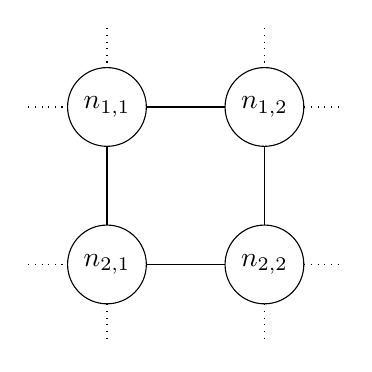
\begin{tikzpicture}[scale=1]
		% Default action for each node
		\tikzstyle{every node}=[draw, shape=circle, minimum size=1cm];

											\coordinate (northleft) at (0, 2);	\coordinate (northright) at (2, 2);
		\coordinate (westup) at (-1,1);		\node (r1c1) at (0,1) {$n_{1,1}$};	\node (r1c2) at (2,1) {$n_{1,2}$};	\coordinate (eastup) at (3,1);
		\coordinate (westdown) at (-1,-1);	\node (r2c1) at (0,-1) {$n_{2,1}$};	\node (r2c2) at (2,-1) {$n_{2,2}$};	\coordinate (eastdown) at (3,-1);
											\coordinate (southleft) at (0, -2);	\coordinate (southright) at (2, -2);

		% Horizontals
		\draw[outside] (westup) -- (r1c1);
		\draw (r1c1) -- (r1c2);
		\draw[outside] (r1c2) -- (eastup);

		\draw[outside] (westdown) -- (r2c1);
		\draw (r2c1) -- (r2c2);
		\draw[outside] (r2c2) -- (eastdown);

		% Verticals
		\draw[outside] (northleft) -- (r1c1);
		\draw (r1c1) -- (r2c1);
		\draw[outside] (r2c1) -- (southleft);

		\draw[outside] (northright) -- (r1c2);
		\draw (r1c2) -- (r2c2);
		\draw[outside] (r2c2) -- (southright);
	\end{tikzpicture}

%% Phase 1 algorithm

\subsubsection{Algorithm}

\begin{enumerate}
\item If $\vinit$ does not have exactly 4 neighbours, that is $ \card{\AdjVV(\vinit)} \neq 4 $, return immediately with $\Structured = \varnothing$.
\item Let $ n_{1,1} = \vinit $, and let $ a, b, c \in \AdjVV(\vinit) $ be distinct vertex neighbours of $\vinit$. Consider vertices $a$ and $b$. If they do not both have exactly 4 neighbours, then they cannot form a part of a structured quad region. Return immediately with $\Structured = \varnothing$.

\item Otherwise, there are three cases:

	%%%% BEGIN THREE CASES
	\begin{enumerate}[label=Case \alph*)]

	%% Straight line case
	\item $a$ and $b$ have exactly one neighbour in common, which must be $n_{1,1}$ by construction, expressed by:
	$$ \card{\AdjVV(a) \cap \AdjVV(b)} = 1$$
	$a, n_{1,1}, b $ are \emph{topologically} along a straight line of a structured grid, and hence cannot form a quad.
	We therefore consider $b$, $n_{1,1}$, and  $c$ instead as candidates, letting $n_{2,1} = b$ and $n_{1,2} = c$.
	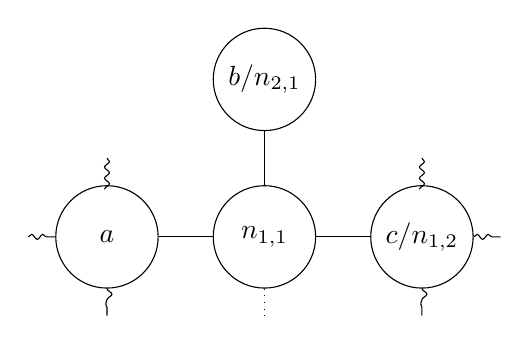
\begin{tikzpicture}
		% Default action for each node
		\tikzstyle{every node}=[draw, shape=circle, minimum size=1.3cm];

										\coordinate (northleft) at (-1,2);	\node (b) at (1,3) {$b / n_{2,1}$};	\coordinate (northright) at (3,2);
		\coordinate (west) at (-2,1);	\node (a) at (-1,1) {$a$};			\node (n11) at (1,1) {$n_{1,1}$};	\node (c) at (3,1) {$c / n_{1,2}$};	\coordinate (east) at (4,1);
										\coordinate (southleft) at (-1,0);	\coordinate (southmid) at (1,0);	\coordinate (southright) at (3,0);

		\draw[anywhere] (west) -- (a);
		\draw (a) -- (n11) -- (c);
		\draw[anywhere] (c) -- (east);

		\draw[anywhere] (northleft) -- (a) -- (southleft);
		\draw (b) -- (n11);
		\draw[outside] (n11) -- (southmid);
		\draw[anywhere] (northright) -- (c) -- (southright);
	\end{tikzpicture}


	%% Angle case
	\item $a$ and $b$ have exactly two neighbours in common, one of which must be $n_{1,1}$ by construction, expressed by:
	$$ \card{\AdjVV(a) \cap \AdjVV(b)} = 2$$
	We continue with vertices $a$, $n_{1,1}$, and $b$ as candidates, letting $n_{2,1} = a$ and $n_{1,2} = b$.
	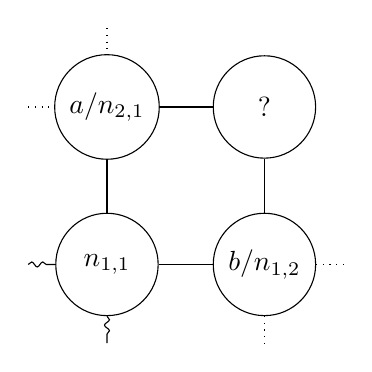
\begin{tikzpicture}
		% Default action for each node
		\tikzstyle{every node}=[draw, shape=circle, minimum size=1.3cm];

											\coordinate (northleft) at (-1,4);		\coordinate (northright) at (1,4);
		\coordinate (westup) at (-2,3);		\node (a) at (-1,3) {$a / n_{2,1}$};	\node (d) at (1,3) {$?$};			\coordinate (eastup) at (2,3);
		\coordinate (westdown) at (-2,1);	\node (n11) at (-1,1) {$n_{1,1}$};		\node (b) at (1,1) {$b / n_{1,2}$};	\coordinate (eastdown) at (2,1);
											\coordinate (southleft) at (-1,0);		\coordinate (southright) at (1,0);



		\draw[outside] (westup) -- (a);
		\draw (a) -- (d);
		% \draw (d) -- (eastup);

		\draw[anywhere] (westdown) -- (n11);
		\draw (n11) -- (b);
		\draw[outside] (b) -- (eastdown);

		\draw[outside] (northleft) -- (a);
		\draw (a) -- (n11);
		\draw[anywhere] (n11) -- (southleft);

		% \draw (northright) -- (d);
		\draw (d) -- (b);
		\draw[outside] (b) -- (southright);

	\end{tikzpicture}


	\item $a$ and $b$ have more than two neighbours in common\footnote{note that the set is non-empty by construction}, expressed by:
	$$ \card{\AdjVV(a) \cap \AdjVV(b)} > 2$$
	We cannot form a quad, and hence return immediately with $\Structured = \varnothing$.

	\end{enumerate}
	%%%% END THREE CASES

\item Find the common neighbours of $n_{2,1}$ and $n_{1,2}$. If there are not exactly two neighbours, return immediately with $\Structured = \varnothing$.

\item One of the two neighbours must be $n_{1,1}$ by construction. Let the other neighbour be $n_{2,2}$

\item Let $N = \{ n_{1,1}, n_{1,2}, n_{2,1}, n_{2,2} \}$. If any vertex $n \in N$ is in $\Visited$, that is $N \cap \Visited \neq \varnothing$, then return immediately with $\Structured = \varnothing$. Otherwise add the vertices in $N$ to $\Visited$.

\item Ensure for every vertex $n \in N$ that its visited neighbours, $\AdjVV(n) \cap \Visited$, are exactly those explicitly stated above. If this is not the case, remove $N$ from $\Visited$ and return immediately with $\Structured = \varnothing$.

\item Set $\Structured = \{ n_{1,1}, n_{1,2}, n_{2,1}, n_{2,2} \}$, and continue to the next phase.

The structured region looks as follows thus far.
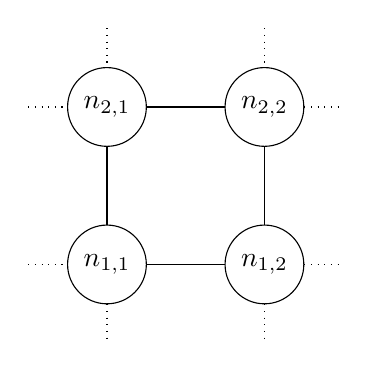
\begin{tikzpicture}
	% Default action for each node
	\tikzstyle{every node}=[draw, shape=circle, minimum size=1cm];

										\coordinate (northleft) at (-1,4);	\coordinate (northright) at (1,4);
	\coordinate (westup) at (-2,3);		\node (n21) at (-1,3) {$n_{2,1}$};	\node (n22) at (1,3) {$n_{2,2}$};	\coordinate (eastup) at (2,3);
	\coordinate (westdown) at (-2,1);	\node (n11) at (-1,1) {$n_{1,1}$};	\node (n12) at (1,1) {$n_{1,2}$};	\coordinate (eastdown) at (2,1);
										\coordinate (southleft) at (-1,0);	\coordinate (southright) at (1,0);



	\draw[outside] (westup) -- (n21);
	\draw (n21) -- (n22);
	\draw[outside] (n22) -- (eastup);

	\draw[outside] (westdown) -- (n11);
	\draw (n11) -- (n12);
	\draw[outside] (n12) -- (eastdown);

	\draw[outside] (northleft) -- (n21);
	\draw (n21) -- (n11);
	\draw[outside] (n11) -- (southleft);

	\draw[outside] (northright) -- (n22);
	\draw (n22) -- (n12);
	\draw[outside] (n12) -- (southright);

\end{tikzpicture}

\end{enumerate}


\chapter{Evaluation}
\label{chap:evaluation}

In this chapter we evaluate various aspects of our work in structure detection.
We first present a technical evaluation of the algorithm, assessing the quality of its output and runtime performance. We also look at the performance characteristics achieved when incorporating our structure detection into the core-computation work-flow.


\section{Benchmarks}
We briefly introduce the sample meshes used as benchmarks.

\subsection{Airfoil grid mesh}
This is a mesh generated using the \texttt{naca0012.m} script~\cite{airfoilgen}, following the NACA0012 definition for constructing an airfoil upper surface. It is parametrised by two variables $I$ and $J$ which denote the length and width of the airfoil boundary. The default airfoil mesh size is is built with $I=400$ and $J=600$, containing about 720,000 vertices. Topologically, the vast majority of the mesh forms a single large rectangular structure. Figure~\ref{fig:airfoil-mesh} shows a sample rendering.

\begin{figure}
\includegraphics[width=\textwidth]{images/evaluation/airfoil.jpeg}
\caption{A rendering of a small sample of the airfoil mesh generated by~\cite{airfoilgen}. The image was obtained from \cite{Tkachov2012thesis}.}
\label{fig:airfoil-mesh}
\end{figure}

\subsection{NACA0012 mesh}
This mesh was generated from \texttt{naca0012.geo}, kindly provided by George Ntemos, using Gmsh~\cite{geuzaine2008gmsh}. It represents the construction of a NACA0012 airfoil at zero incidence. The mesh is fairly coarse, containing roughly 15,000 vertices. Figure~\ref{fig:naca0012-mesh} shows sample renderings.

\begin{figure}
\sidebysidevertical
{
  \includegraphics[width=\textwidth]{images/evaluation/naca0012.pdf}
  \caption{A wide shot of the airfoil.}
}
{
  \includegraphics[width=\textwidth]{images/evaluation/naca0012-closeup.pdf}
  \caption{A close-up at the airfoil border. Note the highly structured region formed directly around the airfoil.}
}
\caption{A rendering of the naca0012 airfoil mesh.}
\label{fig:naca0012-mesh}
\end{figure}

\subsection{NACA0021 mesh}
This mesh was generated from \texttt{naca0021.geo}, kindly provided by Harry Davis, using Gmsh~\cite{geuzaine2008gmsh}. It represents the construction of a NACA0021 airfoil at a 60 degree angle of attack. The mesh contains roughly 20,000 vertices. Figure~\ref{fig:naca0021-mesh} shows sample renderings.

\begin{figure}
\sidebysidevertical
{
  \includegraphics[width=\textwidth]{images/evaluation/naca0021.pdf}
  \caption{A (very) wide shot of the airfoil. The diagonal facing spec in the middle is the airfoil!}
}
{
  \includegraphics[width=\textwidth]{images/evaluation/naca0021-closeup.pdf}
  \caption{A close-up at the airfoil border. Note the large structured region formed behind the airfoil.}
}
\caption{A rendering of the naca0021 airfoil mesh.}
\label{fig:naca0021-mesh}
\end{figure}


\subsection{The airfoil computation}
\label{subsec:airfoil-computation}
The airfoil computation is an example core-computation which is used as an example application in OP2~\cite{op2airfoil}. The computation applies the volume method to solve the 2D Euler equations iteratively, refining the solution until a steady state is reached. Within each iterations it performs multiple loops over cells and meshes, which involve both reading and writing data.

This application serves as a good benchmark, as it allows us to
\begin{enumerate*}[label=\alph*)]
\item compare our performance against OP2's, and
\item compare out computed results against OP2's, to ensure correctness.
\end{enumerate*}

\section{Metrics}
\subsection{Core-computation metrics}
There are three types of core-computation executions which we evaluate:
\begin{itemize}
\item Baseline OP2 execution time
The runtime of the core-computation with OP2~\cite{op2common}, which does not use any structured region information. Mesh elements are accessed using indirection maps.

\item Crystal execution time
The runtime of the core-computation with Crystal using structured region information. Mesh elements in structured regions are accessed directly using address calculations; mesh elements in unstructured regions are accessed using indirection maps.

\item Unstructured Crystal execution time
The runtime of the core-computation with Crystal \emph{without} providing structured region information. Mesh elements are accessed using indirection maps. The structured loops are still present in the code, though they are skipped at runtime due to missing structured region information. In effect, this is a competing implementation of the same iteration algorithm used by OP2.
\end{itemize}
All execution measurements exclude initialization and cleaning up time, which in any case have been found to be negligible.

\subsection{Detection metrics}
\begin{itemize}
\item Structured region size:

This is the number of vertices found in a particular structured region. The general notion may refer to the average of such number.
\item Number of structured regions detected
\item Detection coverage: Either the number or percentage (as defined in context) of vertices in the mesh detected as structured elements.
\end{itemize}


\section{Structure detection}
The first step in evaluating our structure detection algorithms, manifested through our implementation, is to answer the simple question: does it work? Using detection metric here is useful, but at a fundamental level the best way to assess whether the implementation works as expected is to visualise the result.


\subsection{Airfoil grid}
Our first structure detection run is performed on the airfoil grid, as it is the simplest case for which we can assess correctness. Figure~\ref{fig:airfoil-grid-visual} shows the result of running structure detection on a very small version of the airfoil grid mesh. We can clearly see that the structured regions are as we would expect, forming a two-dimensional lattice which spans to include all structured vertices.

\begin{figure}
\includesvg[width=\textwidth, svgpath=images/evaluation/]{airfoil_structure}
\caption[Visualisation of detected structure in the airfoil grid mesh]{A rudimentary visualisation\footnotemark{} of the detected structure in an airfoil grid mesh. The mesh is parametrised with $I=4$ and $J=6$, resulting in 91 vertices. Structured vertices and cells are denoting in bright and dull red, respectively. Note that the numbering shown denotes the old mesh numbering.}
\label{fig:airfoil-grid-visual}
\end{figure}\nopagebreak\footnotetext{The custom \texttt{*.dat} used by the authors of this mesh does not make it amenable to visualisation by popular tools. This image was generated using a Python script outputting a graph description, with suitable colour and label information, which is then passed to the \texttt{dot}~\cite{ellson2002graphviz} utility to visualize.}



\subsection{NACA0012}
We now consider more complex meshes where more interesting patterns of structure can be found. First, we detect the structure in the NACA0012 mesh, depicted in figure~\ref{fig:naca0012-structure}. Notice how the highly structured region surrounding the borders of the airfoil is cleanly detected as one big structured region. However, looking at the small patches of structure, it is clear that there have been some losses. All these losses, however, are distinctly attributable to our choice of length-first search, which we described in subsection~\ref{subsec:length-first-search} as being eager. We shall see an example of this shortly.

Figure~\ref{fig:plot-naca0012-region-sizes} shows the structured region frequency for the NACA0012, averaged over 200 runs. As would be intuitively expected, a small number of large structured regions are discovered, whereas small structured regions are abundant. Structured region size seems to follow a skewed normal distribution, with a peak value at 12.

Figure~\ref{fig:plot-naca0012-node-region-sizes} on the other hand plots the frequency of vertices \emph{belonging to} a structure of a given size. For example, if we partition a mesh into five regions of size 10 and one region of size 100, respectively, then 50 vertices in the mesh belong to a region of size 10, and 100 vertices belong to a region of size 100. Notice how the sizes of structured regions follow a bimodal distribution: they are typically either very small or very large.

\begin{figure}
\sidebysidevertical{
\includegraphics[width=\textwidth]{images/evaluation/naca0012-structure-cropped.pdf}
}
{
\includegraphics[width=\textwidth]{images/evaluation/naca0012-structure-closeup-cropped.pdf}
}
\caption{A visualisation of the detected structure in the NACA0012 mesh.}
\label{fig:naca0012-structure}
\end{figure}


\begin{figure}
\sidebysidevertical
{
\begin{tikzpicture}
  \begin{axis}[
    ybar,
    bar width=0.5mm,
    width=12cm,
    height=5cm,
    % enlarge y limits=0.5,
    xlabel = Structured region size,
	ylabel = Average frequency,
	xmode = log,
    % nodes near coords, nodes near coords align={horizontal},
	legend pos = north west,
    ]
 pos = south east
]


\addplot [
fill=blue!80!white,
% pattern=horizontal lines light blue
] table [
y = frequency,
x = regionsize
] {data-naca0012-region-sizes.tsv};


\end{axis}
\end{tikzpicture}

\caption{Plot of the distribution of structured region sizes.}
\label{fig:plot-naca0012-region-sizes}
}
{
\input{plot-naca0012-nodes-with-region-size}
\caption{Plot of the distribution of structured region sizes to which vertices belong.}
\label{fig:plot-naca0012-node-region-sizes}
}
\caption{Statistics related to the structured region sizes of the NACA0012 mesh.}
\end{figure}




\subsection{NACA0021}
Next we look at the results of structure detection for the NACA0021 mesh, shown in figure~\ref{fig:naca0021-structure}. Interestingly the algorithm failed to detect the obvious targets as a single large chunk, and has instead fragmented it into a few relatively large blocks. Examining the boundaries of this large chunk, we find that it has many ``traps'', that is small portions where an eager structure detection algorithm may extend beyond where its supposed, and then get stuck in a sub-optimal configuration. Figure~\ref{fig:naca0021-good-structure} shows the detected structure when we hand-pick a seed vertex which does not fall into such a ``trap''.





Figure~\ref{fig:plot-naca0021-region-sizes} shows the structured region frequency for the NACA0021, averaged over 200 runs. The results are similar to the NACA0012 results in figure~\ref{fig:plot-naca0012-region-sizes}, and in fact the same peak value of 12 is present here.

Figure~\ref{fig:plot-naca0021-node-region-sizes} shows the frequency of vertices \emph{belonging to} a structure of a given size. It is also similar to the corresponding plot for NACA0012 in figure~\ref{fig:plot-naca0012-node-region-sizes}.


\begin{figure}
\sidebysidevertical{
\includegraphics[width=\textwidth]{images/evaluation/naca0021-structure-cropped.pdf}
}
{
\includegraphics[width=\textwidth]{images/evaluation/naca0021-structure-closeup-cropped.pdf}
}
\caption{A visualisation of the detected structure in the NACA0021 mesh.}
\label{fig:naca0021-structure}
\end{figure}


\begin{figure}
\includegraphics[width=\textwidth]{images/evaluation/naca0021-good-structure-cropped.pdf}
\caption{A visualisation of the detected structure in the NACA0021 mesh when hand-picking a ``good'' seed vertex.}
\label{fig:naca0021-good-structure}
\end{figure}


\begin{figure}
\sidebysidevertical
{
\begin{tikzpicture}
  \begin{axis}[
    ybar,
    bar width=0.5mm,
    width=12cm,
    height=5cm,
    % enlarge y limits=0.5,
    xlabel = Structured region size,
	ylabel = Average frequency,
	xmode = log,
    % nodes near coords, nodes near coords align={horizontal},
	legend pos = north west,
    ]
 pos = south east
]


\addplot [
fill=blue!80!white,
% pattern=horizontal lines light blue
] table [
y = frequency,
x = regionsize
] {data-naca0012-region-sizes.tsv};


\end{axis}
\end{tikzpicture}

\caption{Plot of the distribution of structured region sizes.}
\label{fig:plot-naca0021-region-sizes}
}
{
\input{plot-naca0012-nodes-with-region-size}
\caption{Plot of the distribution of structured region sizes to which vertices belong.}
\label{fig:plot-naca0021-node-region-sizes}
}
\caption{Statistics related to the structured region sizes of the NACA0021 mesh.}
\end{figure}

\section{Core-computation runtime performance}

\subsection{Experimental method}
All experiments are performed on a model HP 800 G1 TWR. The processor is an Intel\textregistered{} Core\texttrademark{} i7-4770 3.40GHz with four physical cores\footnote{Note that the experiments were run serially}, supporting the SSE 4.1/4.2 and  AVX 2.0 instruction sets~\cite{intelprocessor}. The main memory capacity of the machine is 16GB.

The creation of the source mesh, where applicable, is never timed, and Crystal loads and uses the data in-memory as standard arrays. Creation refers to storage of the relevant entity set metadata (number of vertices cells, etc), relation maps, and the associated data (typically spatial coordinates). This non-expensive process involves converting the mesh into a custom data format based on Protocol Buffers~\cite{protocolbuffers} with ZIP compression applied using the Minizip library~\cite{minizip}. Our justification behind this is to offer a simplified programming model for data retrieval, manipulation and storage. To our best knowledge this presents no significant advantage to Crystal, if at all.

The Crystal detection code is written in Python and run using the Python interpreter version 2.7.4~\cite{python}.

The Crystal execution code is compiled using the Intel\textregistered{} C and C++ Compilers version 14.0.2 20140120~\cite{icc} with the following optimization flags set:
\begin{itemize}
\item -xHost
\begin{quote}Generate instructions for the highest instruction set and processor available on the compilation host machine.\end{quote}
\item -static-intel
\begin{quote}Link Intel provided libraries statically.\end{quote}
\item -ipo
\begin{quote}Enable multi-file IP [inter-procedural] optimization between files.\end{quote}
\item -O3
\begin{quote}Optimize for maximum speed and enable more aggressive optimizations that may not improve performance on some programs.\end{quote}
\end{itemize}

The baseline OP2 execution code is compiled using the same version of Intel\textregistered{} C and C++ Compilers using the provided Makefile. We use the sequential CPU-only version (double-precision airfoil\_plain)~\cite{op2airfoil}, compiled by issuing the command \texttt{make airfoil\_seq}. The optimization flags set are as follows:
\begin{itemize}
\item -O3 (as above)
\item -xAVX
\begin{quote}May generate Intel\textregistered{} Advanced Vector Extensions (Intel\textregistered{} AVX), Intel\textregistered{} SSE4.2, SSE4.1, SSSE3, SSE3, SSE2, and SSE instructions for Intel\textregistered{} processors.\end{quote}
\item -parallel
\begin{quote}Enable the auto-parallelizer to generate multi-threaded code for loops that can be safely executed in parallel.\end{quote}
\end{itemize}


\subsection{Impact of input mesh numbering}
\subsubsection{Results}
\begin{figure}
  \centering
  \begin{tikzpicture}
\begin{axis}[
xbar,
flexible yticklabels from table={data-airfoil-numbering.tsv}{category}{},
ytick=data,
% xmin = 0,
% ymin = 0,
ylabel = Renumbering,
xlabel = Runtime,
]


\addplot [
draw=blue,
pattern=horizontal lines light blue
] table [
y expr=\coordindex,
x = baseline
] {data-airfoil-numbering.tsv};

]
\addplot [
draw=black,
pattern=horizontal lines dark blue
] table [
y expr=\coordindex,
x = mine
] {data-airfoil-numbering.tsv};

\end{axis}
\end{tikzpicture}

\caption{the Impact of numbering on various types of executions.}
\label{fig:plot-airfoil-numbering}
\end{figure}

\subsubsection{Crystal versus Baseline}
The performance of Crystal, using structure information or otherwise, is far superior to that of the baseline OP2 run. This difference can be attributed to runtime overheads present in the OP2 implementation, notably the \emph{staging} of data\footnote{Staging is the process of transferring data to a temporary holding location for further processing. Staging is usually performed piecemeal on several blocks of data.}.

\subsubsection{Impact of numbering on Crystal with structure information}
The performance of Crystal, given structure information, is agnostic to the original mesh numbering. This is because the vast majority (99.5\%) of vertices are detected to be part of a single monolithic structured region, which Crystal then renumbers in any case.

\subsubsection{Impact of numbering on Crystal without structure information}
The airfoil grid is almost fully structured \emph{by construction}, and has a very good numbering of its elements. Crystal's structure detection then cannot improve on cache locality, merely introducing a small performance overhead. When different numberings are applied to the mesh, however, Crystal using structure information outperforms its non-structure-based counterpart by a modest 11\% improvement with the METIS numbering, and over twice as fast with random numbering.

As a general discussion point, following several investigations into our implementation, we have determined that vectorisation techniques are failing to apply. We suspect that performing further work on optimising the code can make it amenable to vectorisation, and hence superior in performance even when the original numbering is a good one.
% TODO FUTURE and can form the basis of future works



\section{Detected structure quality}
It is difficult to produce a single definitive metric with which we can unequivocally define the quality of our detected structure. We can, however, look at properties that are in line with that target, and derive useful metrics by combining them.

Percentage of mesh elements detected as structured:
This metric is most useful when we know the maximum value that would be expected or possible.
Without this knowledge, the metric is a one-sided test: a high percentage is a positive sign, whereas a lower percentage is indeterminate.

Structured region size:
Larger structured regions are desirable, but similarly to the previous, the maximum possible size is mesh-dependant and may not be known.

Number of structured regions:
On its own this metric is a tricky one to resolve. It is useful, however, to act as a relative scale for other metrics such as structured region size.




% \section{Running the tool}
% ./detect_multiple_structure.py --max_fail=100 --cepmlls-etc meshes/airfoil.p.part airfoil.p

% bin/mesh-printer structure /tmp/airfoil.p
% /tmp/airfoil.p
% 720000 cells
% 721801 nodes
% 1 structured node regions
%   Region 1: 599 rows x 1199 cols = 718201 nodes
% Total structured nodes: 718201
% Total unstructured nodes: 3600
% 1 structured cell regions
%   Region 1: 598 rows x 1198 rows = 716404 nodes
%     Node row 0 to 598 -- Node col 0 to 1198
%     cell2node offset = 0
%     Compass (Unstructured -> Structured):
%       0 -> 0
%       1 -> 1
%       2 -> 3
%       3 -> 2
% 3596 unstructured cells
% unstructured cells offset = 716404
% 1 structured h_edge regions
%   Region 1: 597 rows x 1197 rows = 714609 nodes
%     Node row 1 to 598 -- Node col 1 to 1198
%     edge2node offset = 0
%     Node compass (Unstructured -> Structured):
%       0 -> 0
%       1 -> 1
%     Cell compass (Unstructured -> Structured):
%       0 -> 0
%       1 -> 1
% 1 structured v_edge regions
%   Region 1: 597 rows x 1197 rows = 714609 nodes
%     Node row 1 to 598 -- Node col 1 to 1198
%     edge2node offset = 714609
%     Node compass (Unstructured -> Structured):
%       0 -> 0
%       1 -> 1
%     Cell compass (Unstructured -> Structured):
%       0 -> 1
%       1 -> 0



% Visualising the airfoil

\chapter{Future works}
This project covered extensive grounds on BLA BLA BLA BLA. With that said, there are plenty of interesting future directions to be pursued, and intriguing tangents to be followed.

\section{Triangular and non-quad meshes}
%% TODO cross reference: In section XXX we claim/discuss how..
Our algorithms are designed to work on meshes with exclusively quadrilateral faces. It is not difficult to imagine modifying the structure detection algorithms to find quadrilateral structure in meshes containing mixed face types such as triangles and hexagons. What would be

We claim that our detection approach can encompass triangle-based structure, and in general any repeating pattern of vertices which may be inscribed in a quadrilateral.


\section{Different types of structure}
Radial, hierarchical
c.f. what I say about polar coordinates
reference hierarchical adaptive mesh refinement, etc

\section{3D meshes}
From surface to volume, in THREE DEE

Could we detect any pattern inscribable in a cube?

\section{Investigate structure growth strategies}
Try the various rectangle growth strategies we outlined.
Try non-rectangular structured regions.
Try different completely techniques (e.g. particle shooting)

Reference particle shooting

\section{Parallelized detection}
That is, detect regions in parallel. Discuss merging regions

Reference particle shooting?


\section{Parallel implementation}
How should we detect and use regions suited for parallel computation?
Likely that we detect the maximum region possible, and then break it down into parts.

Reference the many parallel papers.


\section{Adaptive runtime detection}
Could the detection be performed during runtime, in parallel say. We can hotswap in the structured regions incrementally between iterations as they are detected

Reference the parallel adaptive mesh refinement paper

\section{Geometry based detection}
Could we exploit the underlying geometry to aid in detecting structure?
c.f. Italian paper




\nocite{*} % Show all Bib-entries
\bibliographystyle{plainurl}
\bibliography{thesis}

\end{document}
